\section{Własny zbiór danych}
\label{sec:wlasny-zbior-danych}

\subsection{Opis procesu zbierania danych}
\label{subsec:opis-procesu-zbierania-danych}

Na potrzeby pracy przygotowano własny zbiór próbek pisma odręcznego w języku polskim.
Zbiór został zaprojektowany z myślą o porównaniu modeli rozpoznawania pisma odręcznego,
ze szczególnym uwzględnieniem próbek pochodzących od osób deklarujących dysgrafię.
Dane zbierano z wykorzystaniem papierowych formularzy A4, na których uczestnicy przepisywali
krótkie zdania w sposób naturalny. Nie narzucano tempa pisania, kroju liter ani sposobu
rozmieszczenia tekstu poza prośbą o zapisanie każdej odpowiedzi w jednej linii. W praktyce
część osób wychodziła poza linię pomocniczą albo zapisywała odpowiedź w dwóch wierszach, co
zostało uwzględnione na etapie przetwarzania i walidacji danych.

Formularz zawierał również pola metadanych, obejmujące płeć, rok urodzenia oraz deklarację
dotyczącą trudności w pisaniu. Uczestnik mógł zaznaczyć brak trudności, dysgrafię albo inną
trudność. Informacja o dysgrafii była traktowana jako deklaracja uczestnika, a nie jako diagnoza
kliniczna stawiana na podstawie wyglądu pisma. Takie założenie ogranicza ryzyko subiektywnego
przypisywania uczestników do grupy dysgraficznej wyłącznie na podstawie czytelności pisma.

Przygotowano trzy warianty formularza, oznaczone jako zestaw A, zestaw B oraz zestaw C.
Każdy wariant zawierał osiem zdań do przepisania. Zdania obejmowały polskie znaki diakrytyczne,
interpunkcję, wielkie litery, liczby, adresy, oznaczenia techniczne oraz krótkie komunikaty.
Dzięki temu zbiór nie ogranicza się wyłącznie do prostych zdań literowych, ale zawiera również
elementy typowe dla praktycznych zastosowań systemów OCR/HTR. Na rysunku~\ref{fig:formularz-pusty}
przedstawiono pusty formularz wykorzystany podczas zbierania danych.

\begin{figure}[htbp]
    \centering
    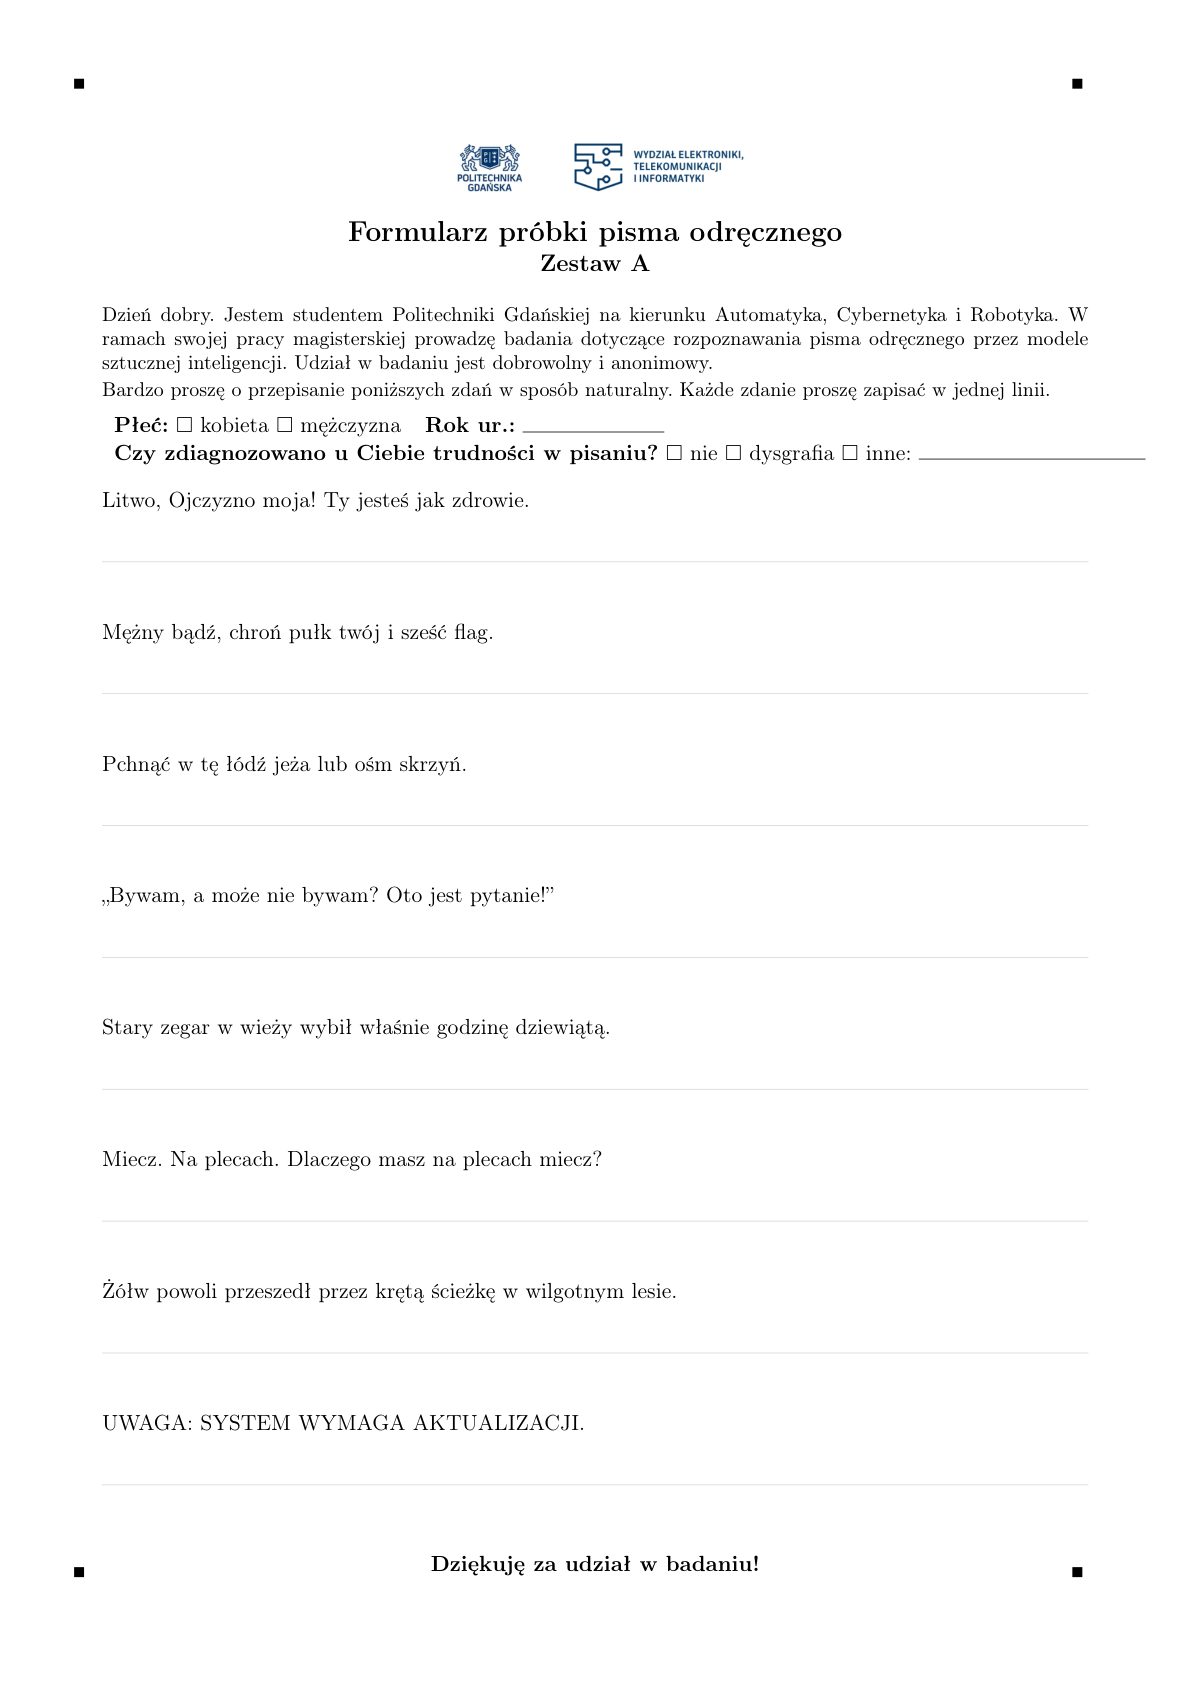
\includegraphics[width=0.72\textwidth]{Formularze/processed_320_check/stats_thesis/figures/formularz_pusty_zestaw_a.png}
    \caption{Pusty formularz wykorzystany do zbierania próbek pisma odręcznego.}
    \label{fig:formularz-pusty}
\end{figure}

W rogach formularzy umieszczono czarne znaczniki geometryczne. Ich zadaniem było ułatwienie
automatycznego wyprostowania zdjęcia lub skanu arkusza. Po digitalizacji formularzy wykrywano
położenie znaczników, a następnie stosowano transformację homograficzną, która sprowadzała
każdy formularz do wspólnego układu współrzędnych. Na tej podstawie wycinano pola metadanych
oraz obszary odpowiadające kolejnym liniom pisma. Wypełniony formularz po normalizacji
geometrycznej przedstawiono na rysunku~\ref{fig:formularz-wypelniony}.

\begin{figure}[htbp]
    \centering
    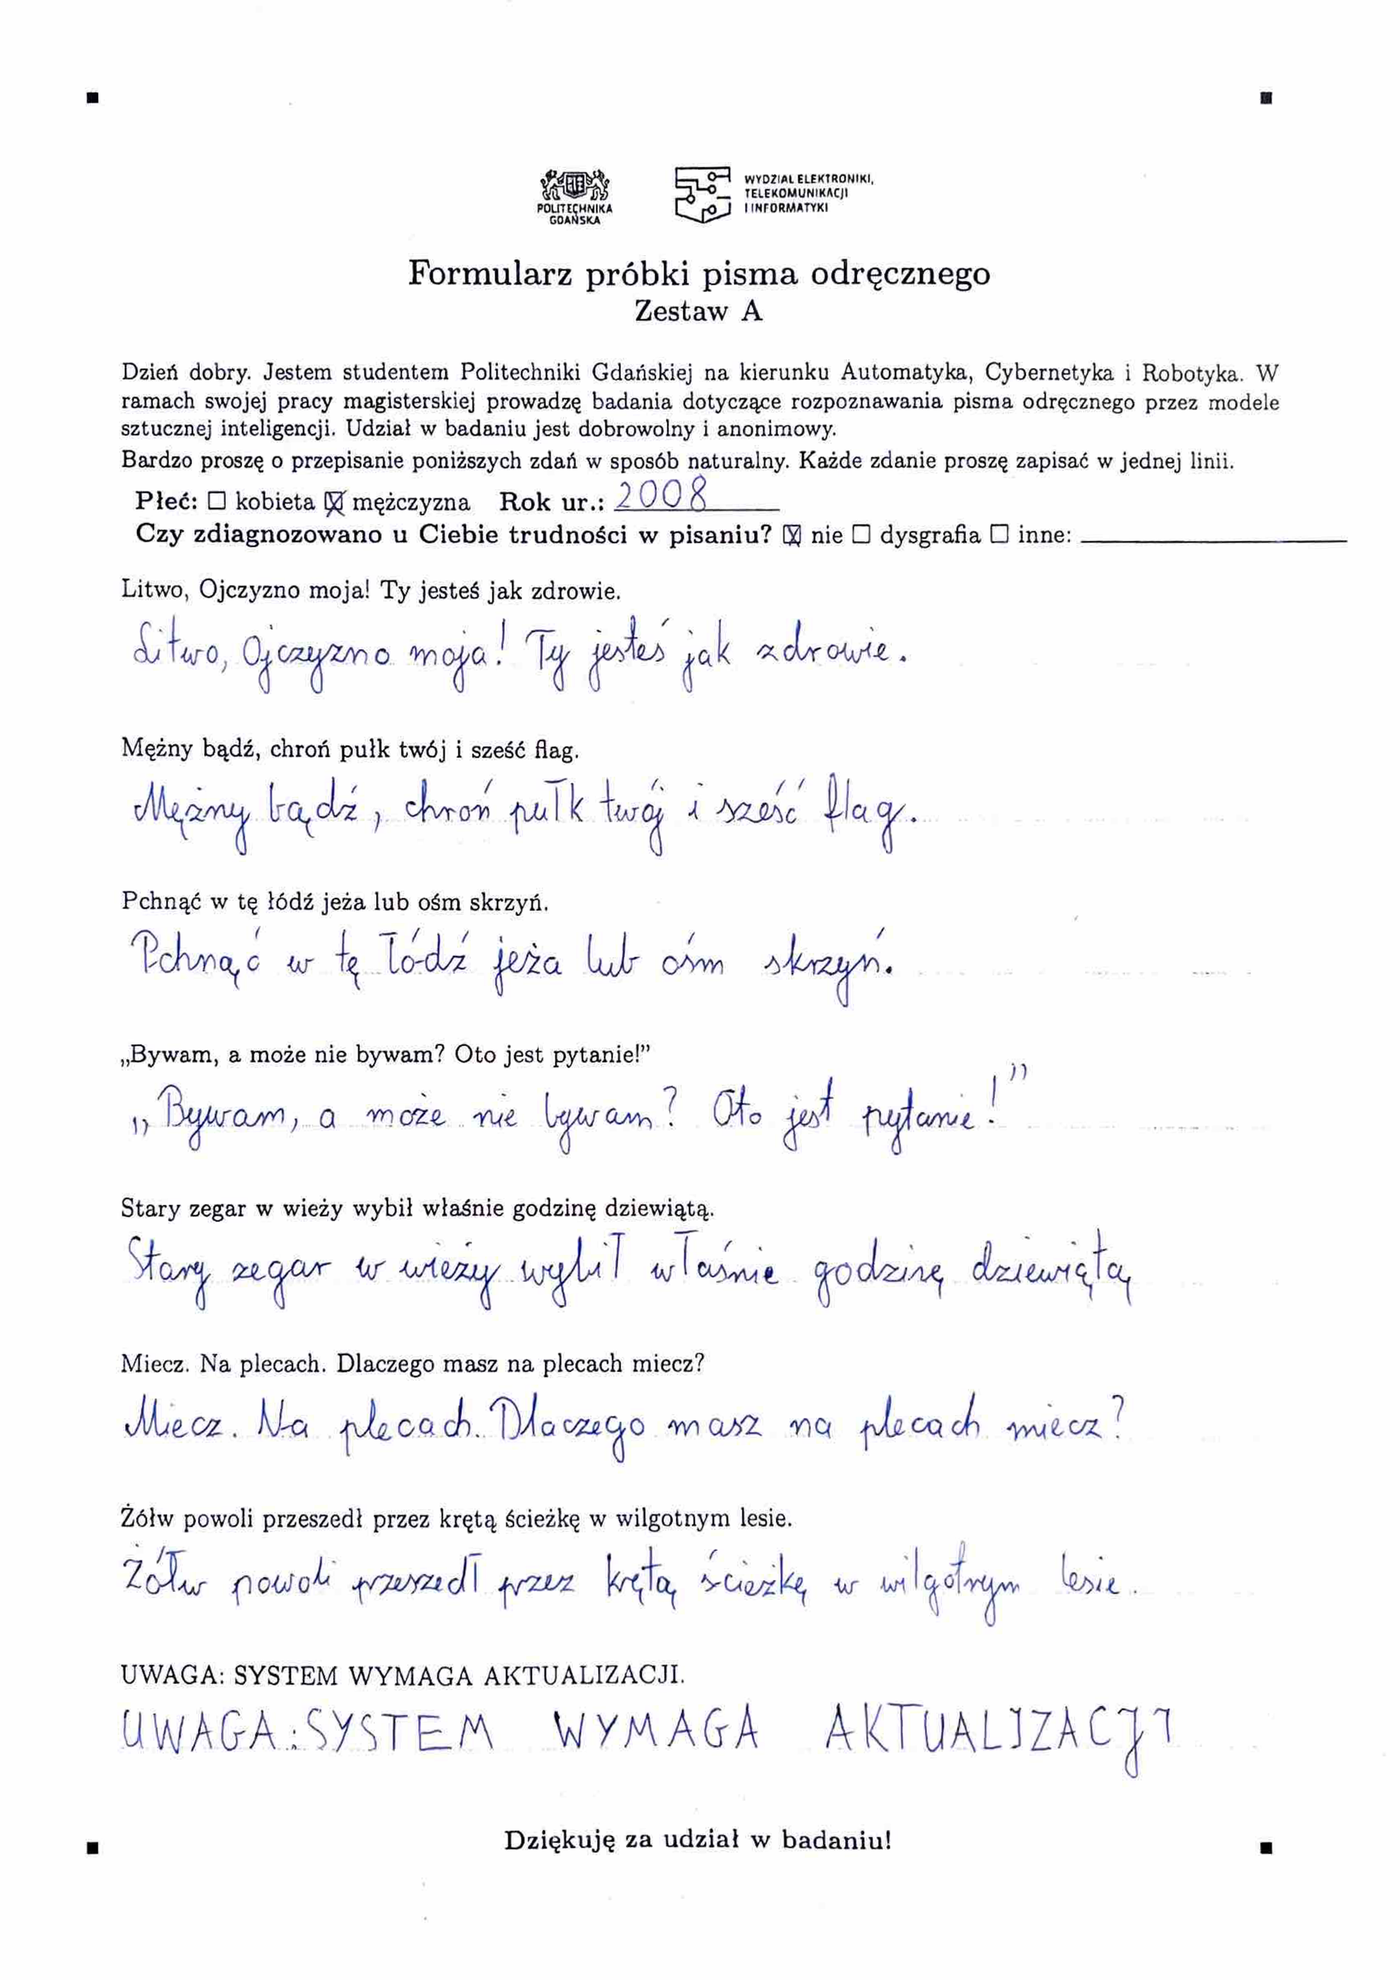
\includegraphics[width=0.72\textwidth]{Formularze/processed_320_check/stats_thesis/figures/formularz_wypelniony_przyklad.png}
    \caption{Wypełniony formularz po wyprostowaniu i normalizacji geometrycznej.}
    \label{fig:formularz-wypelniony}
\end{figure}

Podstawową jednostką danych w eksperymentach była pojedyncza linia pisma, reprezentowana jako
obraz oraz odpowiadająca mu transkrypcja ground truth. Po wstępnym przetwarzaniu przeprowadzono
ręczną walidację zbioru. Sprawdzano poprawność metadanych, jakość wyciętych linii oraz treść
transkrypcji. Jeżeli transkrypcja była niejednoznaczna, próbkę oznaczano jako niepewną. Jeżeli
wycinek był technicznie niepoprawny, zawierał zbyt mało tekstu albo nie pozwalał na rzetelne
przypisanie ground truth, próbkę wykluczano z głównego zbioru. Próbki niepewne i wykluczone
pozostawiono w pełnym manifeście danych, ale nie wykorzystano ich w głównej ewaluacji ilościowej.

\subsection{Charakterystyka grupy badawczej}
\label{subsec:charakterystyka-grupy-badawczej}

Zebrany zbiór obejmuje łącznie 320 formularzy, z których każdy odpowiada jednej osobie badanej.
Rozkład płci przedstawiono w tabeli~\ref{tab:dataset-plec}. Większość formularzy pochodziła od
mężczyzn, którzy stanowili 63{,}12\% uczestników. Kobiety stanowiły 36{,}25\% zbioru, natomiast
w dwóch przypadkach płeć pozostała nieokreślona.

\begin{table}[htbp]
    \centering
    \caption{Rozkład formularzy według płci.}
    \label{tab:dataset-plec}
    \begin{tabular}{lrr}
        \hline
        Płeć & Liczba formularzy & Udział [\%] \\
        \hline
        Mężczyzna & 202 & 63{,}12 \\
        Kobieta & 116 & 36{,}25 \\
        Nieokreślona & 2 & 0{,}62 \\
        \hline
    \end{tabular}
\end{table}

Wiek uczestników określono na podstawie roku urodzenia. Ponieważ nie zbierano dokładnych dat
urodzenia, w analizie wykorzystano wiek rocznikowy, obliczony jako różnica między rokiem 2026
a rokiem urodzenia. Rozkład roczników przedstawiono w tabeli~\ref{tab:dataset-roczniki} oraz
na rysunku~\ref{fig:forms-by-birth-year}. Najliczniejszą grupę stanowili uczestnicy urodzeni
w 2010 roku.

\begin{table}[htbp]
    \centering
    \caption{Rozkład formularzy według roku urodzenia.}
    \label{tab:dataset-roczniki}
    \begin{tabular}{lrr}
        \hline
        Rok urodzenia & Liczba formularzy & Udział [\%] \\
        \hline
        2005 & 3 & 0{,}94 \\
        2006 & 17 & 5{,}31 \\
        2007 & 52 & 16{,}25 \\
        2008 & 52 & 16{,}25 \\
        2009 & 60 & 18{,}75 \\
        2010 & 95 & 29{,}69 \\
        2011 & 14 & 4{,}38 \\
        2012 & 8 & 2{,}50 \\
        2013 & 10 & 3{,}12 \\
        2014 & 8 & 2{,}50 \\
        Nieokreślony & 1 & 0{,}31 \\
        \hline
    \end{tabular}
\end{table}

\begin{figure}[htbp]
    \centering
    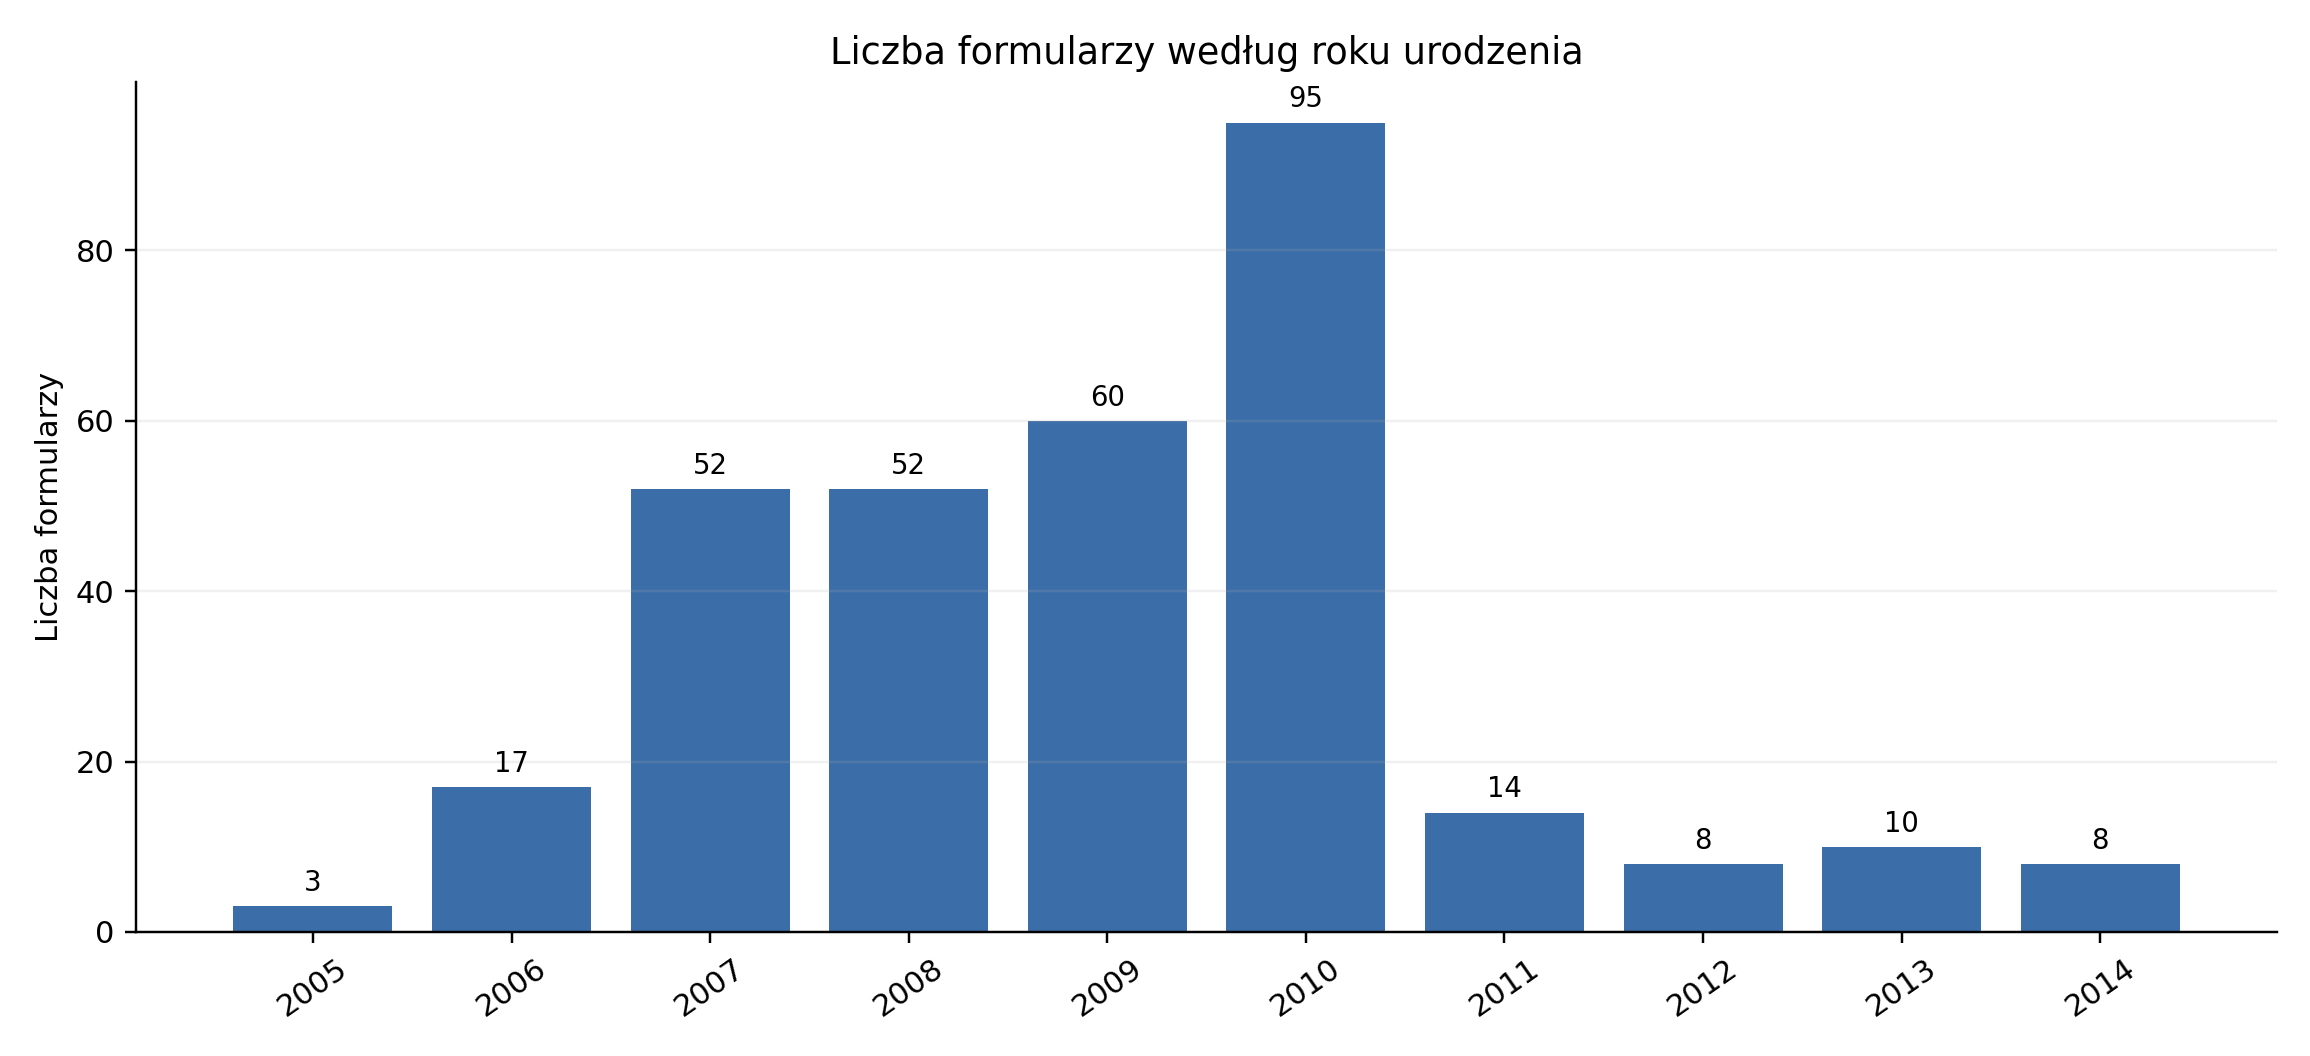
\includegraphics[width=0.82\textwidth]{Formularze/processed_320_check/stats_thesis/figures/forms_by_birth_year.png}
    \caption{Rozkład formularzy według roku urodzenia uczestników.}
    \label{fig:forms-by-birth-year}
\end{figure}

Tabela~\ref{tab:dataset-trudnosci-deklarowane} przedstawia rozkład szczegółowych deklaracji
dotyczących trudności w pisaniu. Największą grupę stanowiły osoby bez zadeklarowanych trudności.
Osoby deklarujące dysgrafię stanowiły 20{,}94\% wszystkich formularzy, natomiast osoby
deklarujące dysleksję 9{,}69\%. W zbiorze wystąpiły również pojedyncze przypadki dysortografii,
innych trudności oraz formularze z nieokreśloną deklaracją.

\begin{table}[htbp]
    \centering
    \caption{Rozkład formularzy według deklarowanej trudności.}
    \label{tab:dataset-trudnosci-deklarowane}
    \begin{tabular}{lrr}
        \hline
        Deklarowana trudność & Liczba formularzy & Udział [\%] \\
        \hline
        Brak trudności & 215 & 67{,}19 \\
        Dysgrafia & 67 & 20{,}94 \\
        Dysleksja & 31 & 9{,}69 \\
        Dysortografia & 2 & 0{,}62 \\
        Inne & 2 & 0{,}62 \\
        Nieokreślone & 3 & 0{,}94 \\
        \hline
    \end{tabular}
\end{table}

Na potrzeby głównej analizy eksperymentalnej szczegółowe deklaracje zagregowano do trzech grup:
brak trudności, dysgrafia oraz inne. Grupa \textit{inne} obejmuje m.in. dysleksję, dysortografię
oraz pozostałe trudności, które nie były analizowane jako osobna kategoria główna.
Rozkład tych grup przedstawiono w tabeli~\ref{tab:dataset-grupy-trudnosci} oraz na
rysunku~\ref{fig:forms-by-difficulty-group}.

\begin{table}[htbp]
    \centering
    \caption{Rozkład formularzy według zagregowanej grupy trudności.}
    \label{tab:dataset-grupy-trudnosci}
    \begin{tabular}{lrr}
        \hline
        Grupa & Liczba formularzy & Udział [\%] \\
        \hline
        Brak trudności & 212 & 66{,}25 \\
        Dysgrafia & 71 & 22{,}19 \\
        Inne & 37 & 11{,}56 \\
        \hline
    \end{tabular}
\end{table}

\begin{figure}[htbp]
    \centering
    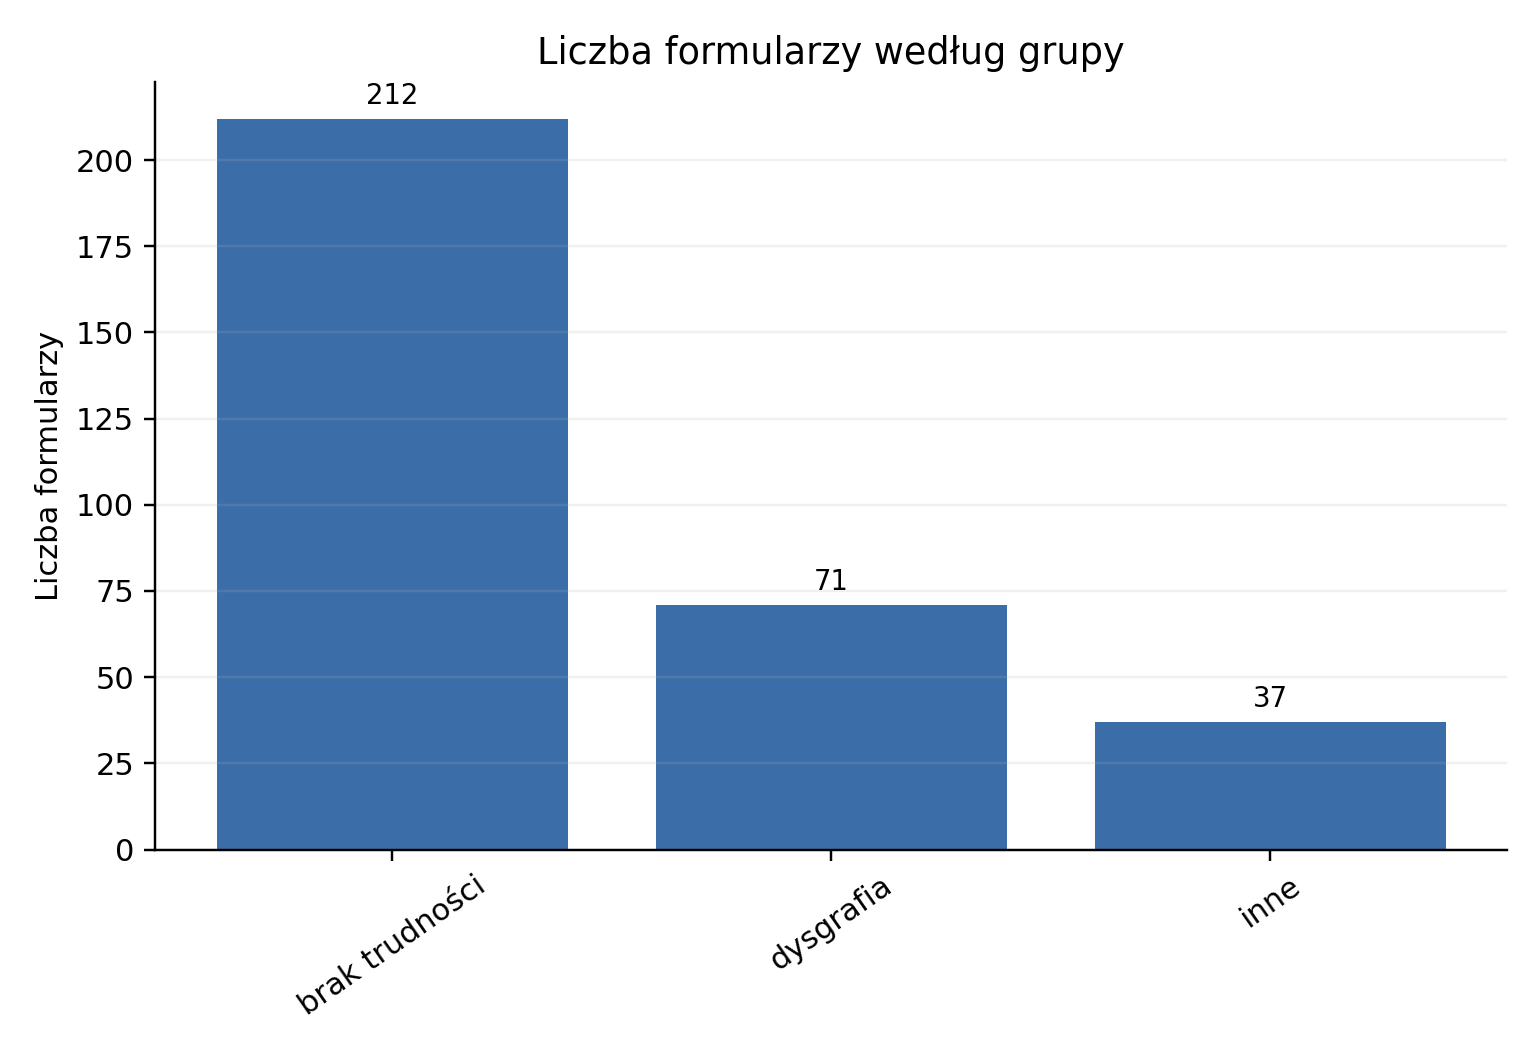
\includegraphics[width=0.74\textwidth]{Formularze/processed_320_check/stats_thesis/figures/forms_by_difficulty_group.png}
    \caption{Rozkład formularzy według zagregowanej grupy trudności.}
    \label{fig:forms-by-difficulty-group}
\end{figure}

\subsection{Struktura i statystyki zbioru}
\label{subsec:struktura-i-statystyki-zbioru}

Każdy formularz zawierał osiem pól przeznaczonych na odpowiedzi, co daje łącznie 2560
potencjalnych próbek liniowych. Po ręcznej walidacji do właściwego zbioru treningowo-testowego
włączono 2313 obrazów linii. Pozostałe 247 slotów nie zostało wyeksportowanych, ponieważ
oznaczono je jako niepewne albo wykluczone. Tabela~\ref{tab:dataset-status-gt} przedstawia
rozkład statusów ground truth po walidacji.

\begin{table}[htbp]
    \centering
    \caption{Status ground truth dla wszystkich slotów linii.}
    \label{tab:dataset-status-gt}
    \begin{tabular}{lrr}
        \hline
        Status GT & Liczba slotów & Udział [\%] \\
        \hline
        OK & 2313 & 90{,}35 \\
        Niepewne & 199 & 7{,}77 \\
        Wyklucz & 48 & 1{,}88 \\
        \hline
    \end{tabular}
\end{table}

Do głównego zbioru danych włączono wyłącznie próbki o statusie \textit{OK}. Próbki oznaczone
jako niepewne pozostawiono w pełnym manifeście, ale nie uwzględniano ich w głównej ewaluacji
ilościowej. Ogranicza to wpływ arbitralnych decyzji anotacyjnych na wartości metryk CER i WER.
Jest to szczególnie istotne w przypadku pisma dysgraficznego, gdzie część próbek może być
trudna do jednoznacznego odczytania nawet dla człowieka.

Tabela~\ref{tab:dataset-obrazy-trudnosci} przedstawia liczbę wyeksportowanych obrazów linii
w podziale na szczegółową deklarację trudności. Po walidacji zbiór zawiera 433 obrazy linii
osób deklarujących dysgrafię oraz 230 obrazów linii osób deklarujących dysleksję.

\begin{table}[htbp]
    \centering
    \caption{Liczba wyeksportowanych obrazów linii według deklarowanej trudności.}
    \label{tab:dataset-obrazy-trudnosci}
    \begin{tabular}{lrr}
        \hline
        Deklarowana trudność & Liczba obrazów linii & Udział [\%] \\
        \hline
        Brak trudności & 1613 & 69{,}74 \\
        Dysgrafia & 433 & 18{,}72 \\
        Dysleksja & 230 & 9{,}94 \\
        Dysortografia & 13 & 0{,}56 \\
        Inne & 7 & 0{,}30 \\
        Nieokreślone & 17 & 0{,}73 \\
        \hline
    \end{tabular}
\end{table}

Po zagregowaniu kategorii do trzech głównych grup otrzymano 1594 obrazy linii w grupie bez
trudności, 458 obrazów linii w grupie dysgrafii oraz 261 obrazów linii w grupie innych trudności.
Rozkład ten przedstawiono w tabeli~\ref{tab:dataset-obrazy-grupy} oraz na
rysunku~\ref{fig:exported-images-by-difficulty-group}.

\begin{table}[htbp]
    \centering
    \caption{Liczba wyeksportowanych obrazów linii według zagregowanej grupy trudności.}
    \label{tab:dataset-obrazy-grupy}
    \begin{tabular}{lrr}
        \hline
        Grupa & Liczba obrazów linii & Udział [\%] \\
        \hline
        Brak trudności & 1594 & 68{,}91 \\
        Dysgrafia & 458 & 19{,}80 \\
        Inne & 261 & 11{,}28 \\
        \hline
    \end{tabular}
\end{table}

\begin{figure}[htbp]
    \centering
    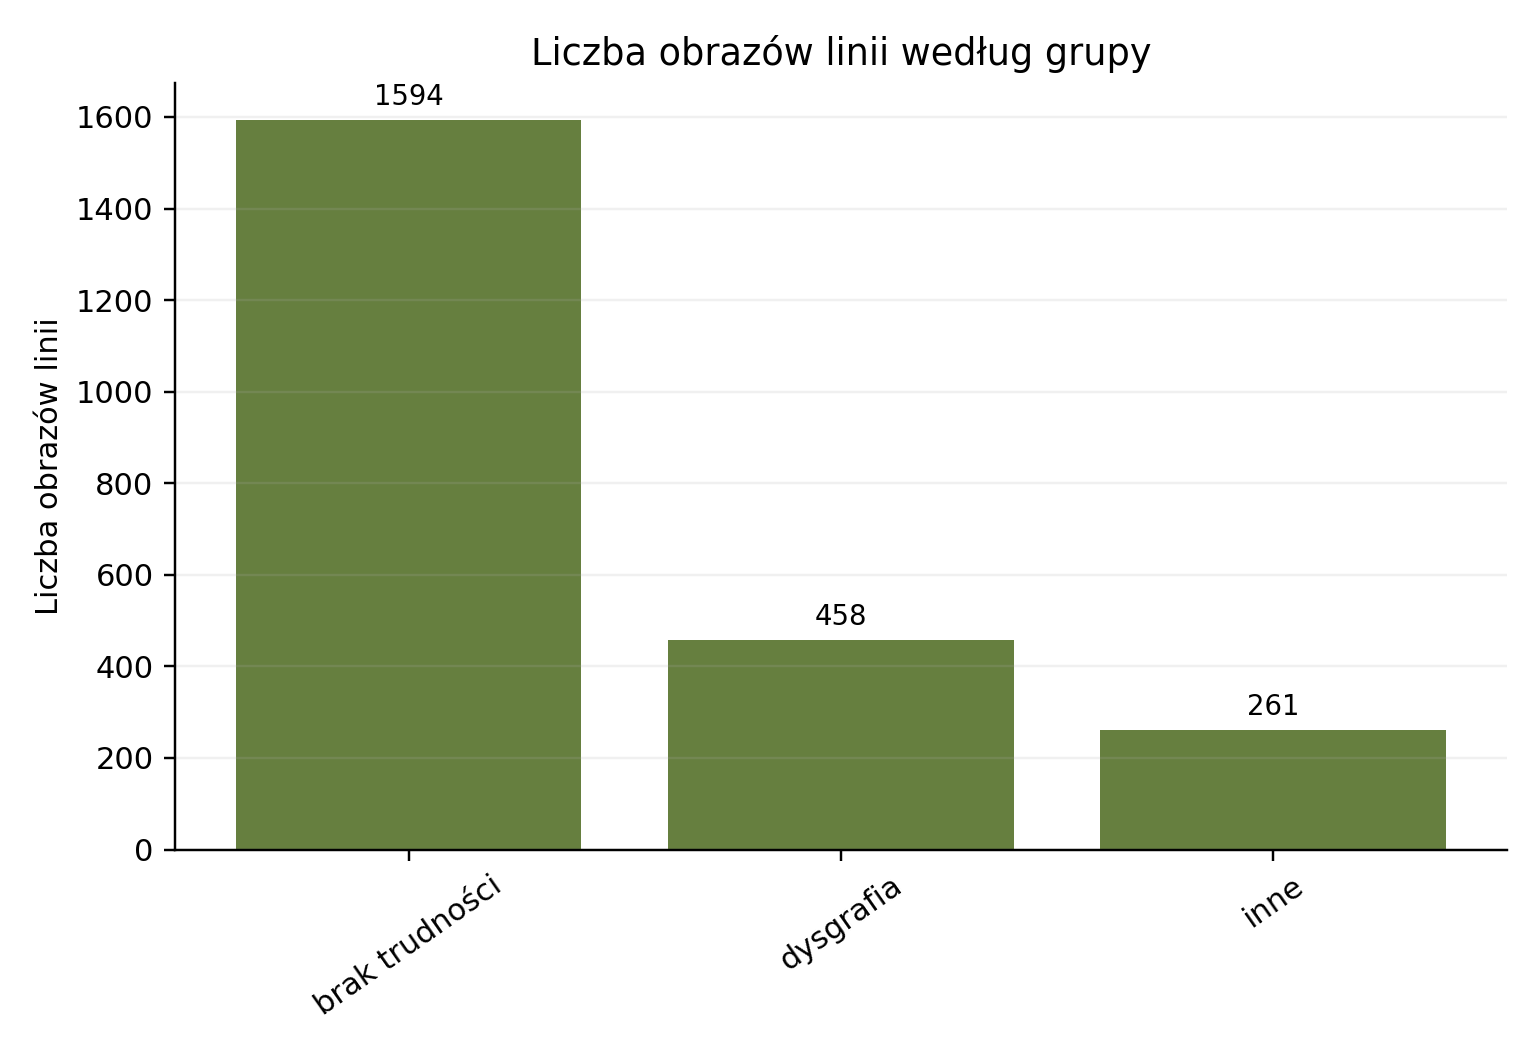
\includegraphics[width=0.74\textwidth]{Formularze/processed_320_check/stats_thesis/figures/exported_images_by_difficulty_group.png}
    \caption{Rozkład wyeksportowanych obrazów linii według zagregowanej grupy trudności.}
    \label{fig:exported-images-by-difficulty-group}
\end{figure}

Zbiór podzielono na część treningową, walidacyjną i testową. Podział wykonano na poziomie
formularza, a więc wszystkie linie jednej osoby przypisano do tego samego splitu. Takie
rozwiązanie zapobiega przeciekowi stylu pisma tej samej osoby między zbiorem treningowym
i testowym. Tabela~\ref{tab:dataset-split} oraz rysunek~\ref{fig:exported-images-by-split}
przedstawiają liczebność poszczególnych części zbioru.

\begin{table}[htbp]
    \centering
    \caption{Podział zbioru na część treningową, walidacyjną i testową.}
    \label{tab:dataset-split}
    \begin{tabular}{lrrrr}
        \hline
        Zbiór & Formularze & Udział form. [\%] & Obrazy linii & Udział obrazów [\%] \\
        \hline
        Train & 254 & 79{,}38 & 1844 & 79{,}72 \\
        Val & 33 & 10{,}31 & 228 & 9{,}86 \\
        Test & 33 & 10{,}31 & 241 & 10{,}42 \\
        \hline
    \end{tabular}
\end{table}

\begin{figure}[htbp]
    \centering
    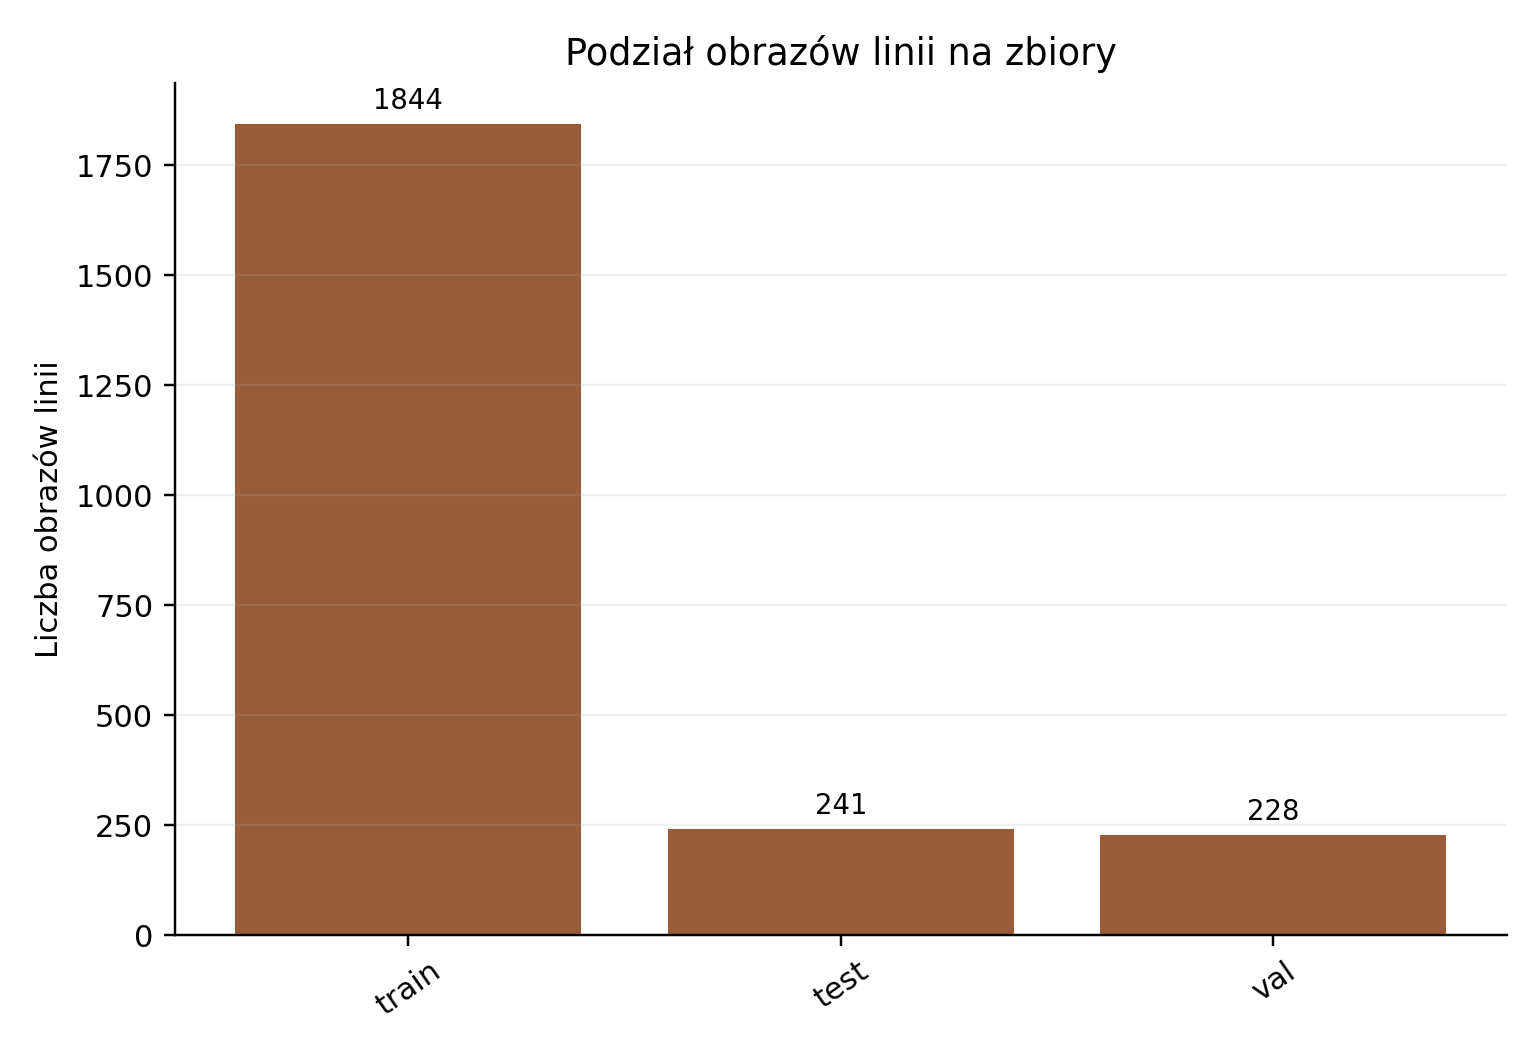
\includegraphics[width=0.72\textwidth]{Formularze/processed_320_check/stats_thesis/figures/exported_images_by_split.png}
    \caption{Podział wyeksportowanych obrazów linii na zbiory treningowy, walidacyjny i testowy.}
    \label{fig:exported-images-by-split}
\end{figure}

Ostateczny zbiór wyeksportowano w formatach dostosowanych do analizowanych modeli. Dla modelu
TrOCR przygotowano pliki CSV zawierające ścieżkę do obrazu i transkrypcję. Dla modelu Qwen
utworzono pliki JSONL zawierające obraz, polecenie transkrypcji oraz odpowiedź referencyjną.
Dla modelu Kraken przygotowano pary plików graficznych i tekstowych, zgodne z konwencją
\texttt{.png} oraz \texttt{.gt.txt}. Każdy z trzech eksportów zawiera 2313 próbek, co potwierdza
spójność przygotowanych formatów danych.
